\documentclass[xetex,mathserif,serif]{beamer}

\usepackage{xunicode}
\usepackage{xltxtra}
\usepackage{color}
\usepackage{url}
\usepackage{listings}
\usepackage{fontspec}
\usepackage{geometry}
\usepackage{lastpage}
\usepackage{fancyhdr}
\usepackage{amsmath}
\usepackage{amsthm}
\usepackage{amssymb}
\usepackage{blkarray}
\usepackage{multicol}
\usepackage{relsize}

\definecolor{solarized@base03}{HTML}{002B36}
\definecolor{solarized@base02}{HTML}{073642}
\definecolor{solarized@base01}{HTML}{586e75}
\definecolor{solarized@base00}{HTML}{657b83}
\definecolor{solarized@base0}{HTML}{839496}
\definecolor{solarized@base1}{HTML}{93a1a1}
\definecolor{solarized@base2}{HTML}{EEE8D5}
\definecolor{solarized@base3}{HTML}{FDF6E3}
\definecolor{solarized@yellow}{HTML}{B58900}
\definecolor{solarized@orange}{HTML}{CB4B16}
\definecolor{solarized@red}{HTML}{DC322F}
\definecolor{solarized@magenta}{HTML}{D33682}
\definecolor{solarized@violet}{HTML}{6C71C4}
\definecolor{solarized@blue}{HTML}{268BD2}
\definecolor{solarized@cyan}{HTML}{2AA198}
\definecolor{solarized@green}{HTML}{859900}
\definecolor{yaleblue}{HTML}{0E4C92}

\newcommand{\yellow}[1]{\textcolor{solarized@yellow}{#1}}
\newcommand{\orange}[1]{\textcolor{solarized@orange}{#1}}
\newcommand{\red}[1]{\textcolor{solarized@red}{#1}}
\newcommand{\magenta}[1]{\textcolor{solarized@magenta}{#1}}
\newcommand{\violet}[1]{\textcolor{solarized@violet}{#1}}
\newcommand{\blue}[1]{\textcolor{solarized@blue}{#1}}
\newcommand{\cyan}[1]{\textcolor{solarized@cyan}{#1}}
\newcommand{\green}[1]{\textcolor{solarized@green}{#1}}
\newcommand{\yblue}[1]{\textcolor{yaleblue}{#1}}

\setbeamertemplate{navigation symbols}{}
% \setbeamerfont{title}{family=\old}
% \setbeamerfont{author}{family=\tfont}%
% \setbeamerfont{frametitle}{family=\oldA}
% \setbeamerfont{date}{family=\dfont}

% \addtobeamertemplate{navigation symbols}{}{%
%     \usebeamerfont{footline}%
%     \usebeamercolor[fg]{footline}%
%     \hspace{1em}%
%     \insertframenumber/\inserttotalframenumber
% }

\setbeamertemplate{footline}[text line]{%
  \parbox{0.99\linewidth}{
    \normalsize\vspace*{-24pt}\hfill{\color{solarized@base00}\insertframenumber/\inserttotalframenumber}
  }
}


\setbeamertemplate{itemize items}{--}
\setbeamercolor*{item}{fg=black}

\defaultfontfeatures{Mapping=tex-text}
\hypersetup{pdfstartview={FitH}}

\newcommand{\old}[1]{\fontspec[Alternate=1,Ligatures={Common}]{Hoefler Text}\fontsize{18pt}{30pt}\selectfont #1}%
\newcommand{\oldA}[1]{\fontspec[Alternate=1,Ligatures={Common, Rare}]{Hoefler Text}\fontsize{12pt}{15pt}\selectfont #1}%
\newcommand{\oldB}[1]{\fontspec[Ligatures={Common}]{Didot}\fontsize{12pt}{15pt}\color{solarized@base02}\selectfont #1}%
\newcommand{\tfont}[1]{\fontspec[Alternate=1,Ligatures={Common}]{Hoefler Text}\fontsize{12pt}{20pt}\selectfont #1}%
\newcommand{\dfont}[1]{\fontspec[Ligatures={Common}]{Didot}\fontsize{12pt}{12pt}\selectfont #1}%

% \newcommand{\minimize}{\mathop{\mathrm{minimize}}}
\newcommand{\argmin}{\mathop{\mathrm{arg\,min}}}
\newcommand{\argmax}{\mathop{\mathrm{arg\,max}}}
\newcommand{\st}{\mathop{\mathrm{subject\,\,to}}}

\newcommand\independent{\protect\mathpalette{\protect\independenT}{\perp}}
\def\independenT#1#2{\mathrel{\rlap{$#1#2$}\mkern2mu{#1#2}}}

\setlength{\parindent}{0pt}
\setlength{\parskip}{12pt}

\setromanfont [Ligatures={Common}, Numbers={OldStyle}, Variant=01,
 BoldFont={LinLibertine_RB.otf},
 ItalicFont={LinLibertine_RI.otf},
 BoldItalicFont={LinLibertine_RBI.otf}
 ]{LinLibertine_R.otf}



\newcommand{\blueone}{{\color{yaleblue} 1}}
\newcommand{\greyzero}{{\color{solarized@base00} 0}}
\usepackage{sty/personalmacros}
\usepackage{sty/personalslides}

\begin{document}
\title{Senior Thesis: Midterm Presentation}
%%%%%%%%%%%%%%%%%%%%%%%%%%%%%%%%%%%%%%%%%%%%%%%%%%%%%%%%%%%%%%%%%%%%%%%%%%%%%%%
% Manifest
% --------
% - Title
% - Outline
% - Review of Graphical Models
% - Review of Multivariate Gaussian
% - Precision Matrices in Context of Gaussian Graphical Models
% - Pairwise Inference for Entrywise Recovery
% - Upper Bound ($\ell_infty$ norm)
%   - Statement of Theorems 2 and 3
%   - Proof / Intuition for Theorems 2 and 3
% - Lower Bound ($\ell_infty$ norm)
%   - Statement of Theorem 5
%   - Proof / Intuition for Theorem 5
% - Next Steps
%%%%%%%%%%%%%%%%%%%%%%%%%%%%%%%%%%%%%%%%%%%%%%%%%%%%%%%%%%%%%%%%%%%%%%%%%%%%%%%
\begin{frame}[fragile] \frametitle{}
\vfill
\vspace{0.2cm}
{
    \color{yaleblue}
    \fontsize{0.5cm}{0cm}\selectfont
    Midterm Presentation: \\
}
\vspace{1.0cm}
{
    \fontsize{0.7cm}{0cm}\selectfont
    Risk Properties in Bandable Precision Matrix Estimation\\
}

\hfill

\vspace{1.8cm}
\begin{minipage}{1.0\textwidth}\raggedleft
    \color{yaleblue}
    Addison Hu   \\
    Statistics 490 \\
    01 March 2017
\end{minipage}
\end{frame}
%%%%%%%%%%%%%%%%%%%%%%%%%%%%%%%%%%%%%%%%%%%%%%%%%%%%%%%%%%%%%%%%%%%%%%%%%%%%%%%
% Outline
%%%%%%%%%%%%%%%%%%%%%%%%%%%%%%%%%%%%%%%%%%%%%%%%%%%%%%%%%%%%%%%%%%%%%%%%%%%%%%%
\begin{frame}[fragile] \frametitle{}
    \slideheader{Outline}
    \begin{enumerate}
        \item Refresher on Graphical Models \& Multivariate Gaussian
        \item Pairwise Inference for Entrywise Recovery of $\Sigma^{-1}$
        \item Risk Bounds for Entrywise Recovery in $\norm{\cdot}_\infty$
        \item Next Steps
    \end{enumerate}
\end{frame}
%%%%%%%%%%%%%%%%%%%%%%%%%%%%%%%%%%%%%%%%%%%%%%%%%%%%%%%%%%%%%%%%%%%%%%%%%%%%%%%
% Refresher
%%%%%%%%%%%%%%%%%%%%%%%%%%%%%%%%%%%%%%%%%%%%%%%%%%%%%%%%%%%%%%%%%%%%%%%%%%%%%%%
\begin{frame}[fragile] \frametitle{}
    \sectionslide{Refresher}
\end{frame}
%%%%%%%%%%%%%%%%%%%%%%%%%%%%%%%%%%%%%%%%%%%%%%%%%%%%%%%%%%%%%%%%%%%%%%%%%%%%%%%
\begin{frame}[fragile] \frametitle{}
    \slideheader{Graphical Models}
    \begin{itemize}
        \item Graphical models provide a framework within which to consider
            dependence structure within a group of variables.
        \item In doing so, we may relax the i.i.d. assumption and still perform
            inference feasibly.
        \item Examples:
            \begin{itemize}
                \item Facebook users graph
                \item Gene interaction networks
            \end{itemize}
    \end{itemize}
\end{frame}
%%%%%%%%%%%%%%%%%%%%%%%%%%%%%%%%%%%%%%%%%%%%%%%%%%%%%%%%%%%%%%%%%%%%%%%%%%%%%%%
\begin{frame}[fragile] \frametitle{}
    \slideheader{Markov Random Fields}
    \begin{itemize}
        \item Consider a graph $G = (V, E)$, and a corresponding set of
            random variables $\{X_i\}_{i=1}^{|V|}$, where the random variables
            are indexed by $u \in V$.
        \item \textbf{Pairwise Markov property:} $X_u \indep X_v | X_{V
            \setminus\{u, v\}}$ for any two non-adjacency nodes $u, v$.
        \item \textbf{Local Markov property:} $X_u \indep X_{V \setminus
            \mathrm{cl}(u)} | X_{\mathrm{nb}(u)}$ for any node $v$.
        \item \textbf{Global Markov property:} $X_A \indep X_B | X_S$ for
            disjoint $A, B \subset V$, and a separating subset $S$.
        \item Inference is easy when the edges are known; but is more
            interesting when they are unknown.
    \end{itemize}
    % https://en.wikipedia.org/wiki/Markov_random_field
\end{frame}
%%%%%%%%%%%%%%%%%%%%%%%%%%%%%%%%%%%%%%%%%%%%%%%%%%%%%%%%%%%%%%%%%%%%%%%%%%%%%%%
\begin{frame}[fragile] \frametitle{}
    \slideheader{Example: Hub and Spoke Model}
    \vspace{1cm}
    \begin{columns}[T]
        \begin{column}{.48\textwidth}
            $$
            \bmat{
                \blueone & \greyzero & \greyzero & \blueone & \greyzero &
                \greyzero & \greyzero   \\ 
                \greyzero & \blueone & \greyzero & \blueone & \greyzero &
                \greyzero & \greyzero   \\ 
                \greyzero & \greyzero & \blueone & \blueone & \greyzero &
                \greyzero & \greyzero   \\ 
                \blueone & \blueone & \blueone & \blueone & \blueone & \blueone
                & \blueone   \\ 
                \greyzero & \greyzero & \greyzero & \blueone & \blueone &
                \greyzero & \greyzero   \\ 
                \greyzero & \greyzero & \greyzero & \blueone & \greyzero &
                \blueone & \greyzero   \\ 
                \greyzero & \greyzero & \greyzero & \blueone & \greyzero &
                \greyzero & \blueone
            }
            $$
        \end{column}
        \hfill
        \begin{column}{.48\textwidth}
            \vspace{-0.2cm}
            \hspace{-0.5cm}
            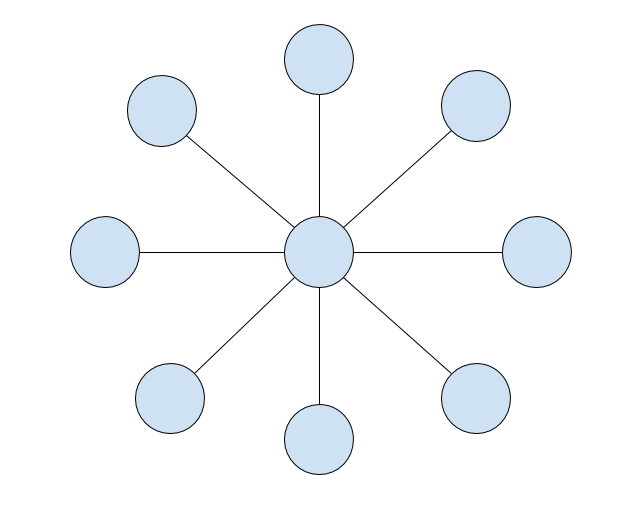
\includegraphics[scale=0.25]{img/spokes.png}
        \end{column}
    \end{columns}
\end{frame}
%%%%%%%%%%%%%%%%%%%%%%%%%%%%%%%%%%%%%%%%%%%%%%%%%%%%%%%%%%%%%%%%%%%%%%%%%%%%%%%
\begin{frame}[fragile] \frametitle{}
    \slideheader{Multivariate Gaussian}

    Suppose $X \dist \Nn(\mu, \Sigma)$. Its density function is given by:
	$$
    p(\xx) = \left(2\pi\right)^{-\frac{p}{2}}\left|\Sigma\right|^{-\frac{1}{2}}
    \exp\lc-\frac{1}{2}(\xx - \mathbf{\mu})^\top \Sigma^{-1}
    (\xx - \mathbf{\mu})\rc
    $$
    \vspace{-0.7cm}
    \begin{itemize}
        \item Closure properties:
            \begin{itemize}
                \item Sum of independent Gaussian random variables is Gaussian.
                \item Marginal of a joint Gaussian distribution is Gaussian.
                \item Condition of a joint Gaussian distribution is Gaussian.
            \end{itemize}
        \item The sparsity pattern of $\Sigma^{-1}$ concides with the adjacency
            matrix of the associated MRF.
    \end{itemize}
    % http://cs229.stanford.edu/section/more_on_gaussians.pdf
\end{frame}
%%%%%%%%%%%%%%%%%%%%%%%%%%%%%%%%%%%%%%%%%%%%%%%%%%%%%%%%%%%%%%%%%%%%%%%%%%%%%%%
\begin{frame}[fragile] \frametitle{}
    \slideheader{Multivariate Gaussian, cont.}

	\begin{itemize}
        \item Closure under marginalization:  Suppose $A \subset V$.  Then
            $$
            \Sigma_{A} = \lp\Sigma_{ij}\rp_{i\in A, j \in A}
            $$
        \item Closure under conditioning: Suppose  $A, B \subset V$, $A \cup B
            = V, A \cap B = \varnothing$.  Then:
            \begin{align*}
                \lp \Omega_A \rp ^{-1}  &= \Sigma_{A|B}   \\
                \lp \Sigma_A \rp ^{-1}  &= \Omega_{A|B}   \\
            \end{align*}
	\end{itemize}
\end{frame}
%%%%%%%%%%%%%%%%%%%%%%%%%%%%%%%%%%%%%%%%%%%%%%%%%%%%%%%%%%%%%%%%%%%%%%%%%%%%%%%
% Pairwise Recovery
%%%%%%%%%%%%%%%%%%%%%%%%%%%%%%%%%%%%%%%%%%%%%%%%%%%%%%%%%%%%%%%%%%%%%%%%%%%%%%%
\begin{frame}[fragile] \frametitle{}
    \sectionslide{Precision Matrix Estimation}
\end{frame}
%%%%%%%%%%%%%%%%%%%%%%%%%%%%%%%%%%%%%%%%%%%%%%%%%%%%%%%%%%%%%%%%%%%%%%%%%%%%%%%
\begin{frame}[fragile] \frametitle{}
    \slideheader{Maximum Likelihood Estimation}

    Assume $\mu = 0$.  Then the maximum likelihood estimation problem is:
	\begin{align*}
		\maximize{
			-\log\det|\Sigma| - \langle \hat\Sigma, \Sigma^{-1} \rangle
		}{\Sigma}{\Sigma \gengeq 0}
	\end{align*}
    \begin{itemize}
        \item Maximum Likelihood Estimate given by $\hat\Sigma = 
            \frac{1}{n} \XX^\top \XX$.
        \item Idea: $\hat\Omega = \hat\Sigma^{-1}$.
        \item Issues:
            \begin{itemize}
                \item Invertibility \& Conditioning
                \item Noise \& Sparsity
            \end{itemize}
    \end{itemize}
\end{frame}
%%%%%%%%%%%%%%%%%%%%%%%%%%%%%%%%%%%%%%%%%%%%%%%%%%%%%%%%%%%%%%%%%%%%%%%%%%%%%%%
\begin{frame}[fragile] \frametitle{}
    \slideheader{Graphical Lasso}

    To encourage sparsity, Tibshirani \textit{et al} proposed imposing an
    entrywise $\ell_1$ penalty on $\Omega$.

    \begin{align*}
        \maximize{
            \log\det|\Omega| - \langle \hat\Sigma, \Omega \rangle
            - \rho \norm{\Omega}_1
        }{\Omega}{\Omega \gengeq 0}
    \end{align*}
\end{frame}
%%%%%%%%%%%%%%%%%%%%%%%%%%%%%%%%%%%%%%%%%%%%%%%%%%%%%%%%%%%%%%%%%%%%%%%%%%%%%%%
\begin{frame}[fragile] \frametitle{}
    \slideheader{Asymptotic Normal Thresholding (ANT)}
    \begin{itemize}
        \item Goal: Obtain entrywise estimates $\hat\omega_{ij}$ of $\Omega$
            that are asymptotically norm and minimax, and then threshold to
            enforce sparsity.
        \item Idea: For each pair $A = \{i, j\}$, regress the variables $X_i,
            X_j$ on all other variables:
            $$
            \XX_A = \XX_{A^c}\beta + \epsilon_A
            $$
            where $\epsilon_A$ is a noise term, distributed normally with mean
            zero, and which are independent of $A^c$.
        \item Rationale: $\Omega_{A, A} = \Sigma_{A|A^c} = \var(X_A|X_{A^c})
            = \var(\epsilon_A)$.  Errors give entries of precision matrix.
    \end{itemize}
\end{frame}
%%%%%%%%%%%%%%%%%%%%%%%%%%%%%%%%%%%%%%%%%%%%%%%%%%%%%%%%%%%%%%%%%%%%%%%%%%%%%%%
\begin{frame}[fragile] \frametitle{}
    \slideheader{Oracle MLE}

    \begin{itemize}
        \item Suppose we could draw from the distribution of $\epsilon_A$
            directly.  How would we estimate $\Omega_{A, A}$?  
        \item The maximum likelihood estimator in this case is:
            $$
            \Theta^{ora}_{A, A} = (\theta^{ora}_{kl})_{k, l \in A}
            = \frac{\epsilon_A^\top\epsilon_A}{n}
            $$
            where we call $\Theta^{ora}$ the \textit{oracle} MLE covariance estimates.
        \item The corresponding oracle MLE precision estimates are then given
            by:
            $$
            \Omega^{ora}_{A, A} = (\omega^{ora}_{kl})_{k, l \in A}
                = \left(\Theta^{ora}_{A, A}\right)^{-1}
            $$
    \end{itemize}
\end{frame}
%%%%%%%%%%%%%%%%%%%%%%%%%%%%%%%%%%%%%%%%%%%%%%%%%%%%%%%%%%%%%%%%%%%%%%%%%%%%%%%
\begin{frame}[fragile] \frametitle{}
    \slideheader{Residual Estimates}
    \begin{itemize}
        \item In practice, we only observe $\XX$, so we must estimate
            $\epsilon_A$.
        \item Suppose we have an adequate estimates of the regression weights
            $\hat\beta$.  Then:
            $$
            \hat\epsilon_A = \XX_A - \XX_{A^c}\hat\beta
            $$
        \item Consequently:
            \vspace{-0.1cm}
            \begin{align*}
                \hat\Theta_{A, A}
                &= \frac{\hat\epsilon_A^\top\hat\epsilon_A}{n}    \\
                \hat\Omega_{A, A} &= \hat\Theta_{A, A}^{-1}
            \end{align*}
    \end{itemize}
\end{frame}
%%%%%%%%%%%%%%%%%%%%%%%%%%%%%%%%%%%%%%%%%%%%%%%%%%%%%%%%%%%%%%%%%%%%%%%%%%%%%%%
\begin{frame}[fragile] \frametitle{}
	\slideheader{Scaled Lasso Estimator}

    For each $m \in A = \{i, j\}$, perform the optimization: 

    $$
    \left\{\hat\beta_m, \hat\theta^{1/2}_{mm}\right\}
    =
    \arg\min_{\substack{b\in\RR^{p-2},\\\sigma \in \RR^+}}
    \left\{
    \frac{\norm{\XX_m - \XX_{A^c}b}^2}{2n\sigma}
    + \frac{\sigma}{2} 
    + \lambda\sum_{k\in A^c}\frac{\norm{\XX_k}}{\sqrt{n}}|b_k|
    \right\}
    $$
    
    Intuitively, the scaling factor on the $\ell_1$ penalty implicitly standardizes
    the design vector to length $\sqrt{n}$ such that the $\ell_1$ penalty is
    applied to the new coefficients $\frac{\norm{\XX_k}}{\sqrt n}b_k$.

\end{frame}
%%%%%%%%%%%%%%%%%%%%%%%%%%%%%%%%%%%%%%%%%%%%%%%%%%%%%%%%%%%%%%%%%%%%%%%%%%%%%%%
% Risk Bounds
%%%%%%%%%%%%%%%%%%%%%%%%%%%%%%%%%%%%%%%%%%%%%%%%%%%%%%%%%%%%%%%%%%%%%%%%%%%%%%%
\begin{frame}[fragile] \frametitle{}
    \sectionslide{Risk Bounds in $\norm{\cdot}_\infty$}
\end{frame}
%%%%%%%%%%%%%%%%%%%%%%%%%%%%%%%%%%%%%%%%%%%%%%%%%%%%%%%%%%%%%%%%%%%%%%%%%%%%%%%
\begin{frame}[fragile] \frametitle{}
    \slideheader{Risk Upper Bound}

    \begin{itemize}
        \item A risk upper bound on an estimator gives a guarantee on its
            worst case performance.
    \end{itemize}
\end{frame}
%%%%%%%%%%%%%%%%%%%%%%%%%%%%%%%%%%%%%%%%%%%%%%%%%%%%%%%%%%%%%%%%%%%%%%%%%%%%%%%
\begin{frame}[fragile] \frametitle{}
    \slideheader{Oracle Inequalities}
\end{frame}
%%%%%%%%%%%%%%%%%%%%%%%%%%%%%%%%%%%%%%%%%%%%%%%%%%%%%%%%%%%%%%%%%%%%%%%%%%%%%%%
\begin{frame}[fragile] \frametitle{}
    \slideheader{Coupling Argument}
\end{frame}
%%%%%%%%%%%%%%%%%%%%%%%%%%%%%%%%%%%%%%%%%%%%%%%%%%%%%%%%%%%%%%%%%%%%%%%%%%%%%%%
\begin{frame}[fragile] \frametitle{}
    \slideheader{Risk Lower Bound}
\end{frame}
%%%%%%%%%%%%%%%%%%%%%%%%%%%%%%%%%%%%%%%%%%%%%%%%%%%%%%%%%%%%%%%%%%%%%%%%%%%%%%%
\begin{frame}[fragile] \frametitle{}
    \slideheader{Le Cam's Two-Point Argument}
\end{frame}
%%%%%%%%%%%%%%%%%%%%%%%%%%%%%%%%%%%%%%%%%%%%%%%%%%%%%%%%%%%%%%%%%%%%%%%%%%%%%%%
\begin{frame}[fragile] \frametitle{}
    \sectionslide{Next Steps}
\end{frame}
%%%%%%%%%%%%%%%%%%%%%%%%%%%%%%%%%%%%%%%%%%%%%%%%%%%%%%%%%%%%%%%%%%%%%%%%%%%%%%%
\end{document}

